\documentclass{hw}
\usepackage{graphicx,listings,xcolor,amsmath,circuitikz}
\title{Lab 3}
\course{ECEN 2270}
\author{Patrick Harrington\\ Bill Fischer}
\date{\today}
\renewcommand\thepart{\Alph{part}}
% Preamble Later
\begin{document}
\maketitle
\abstract{
In this lab, we continue to build on the robot's motor 
functionality. In Part A, we built a DC Motor Driver. 
This addition permits for forward and reverse rotation of the 
wheels. 
In Part B, we created a simple Speed Control circuit. These new 
parts allow for reliable control of the robot's speed and
direction. This is essential in order for the robot to move from 
place to place in a precise and useful way.}

% Part A: DC Motor Driver
\part{DC Motor Driver Circuit}
Building on the Speed Sensor from Lab 2, two DC Motor Driver circuits were
built. Resistors $R_{B1}$ and $R_{B2}$ were calculated and then tested. This
part of the circuit has the following expected parameters:
\begin{itemize}
  \item $V_{BE_{1,4}}\approx0.8[V]$
  \item $\beta\approx200$
  \item $I_{DC}\leq1[A]$
\item $R_M=2[\Omega]$
  \item $V_{CC}=10[V]$
  \item $R_{B1}=R_{B2}=R_B$
  \end{itemize}
This lab also builds on previous findings:
\begin{itemize}
  \item $k=0.927$
  \item $f_{enc_{max}}=1.214[kHz]$
  \item $J=2.61*10^{-3}$
  \item $t_{on}=\frac{3}{4 f_{enc_{max}}}$
  \end{itemize}
\section{Constructing DC Motor Circuit}
Using the proto board supplied, the BJTs were placed onto the board and
connections were soldered such that the connections matched the provided
schematic for the motor driver circuit. 
%Include image? Include sketch of the connections?

\section{Finding $R_B$}
\subsection{$R_B$ by hand}
The specifications for $R_B$ are simple; $|I_{DC}|<1[A]$ if $ V_{DC~
Supply}= 10[V]$. Also, $R_{B1}=R_{B2}=R_B$. The outputs from the driver,
$DC_1$ and $DC_2$, should have a total of $|1[A]|$ through the terminals if the
wheels are locked. When the wheels are locked, the DC Motor from previous labs
acts like a plain old $2[\Omega]$ resistor.


%Model of motor driver
\begin{figure}[ht!]
  \centering
  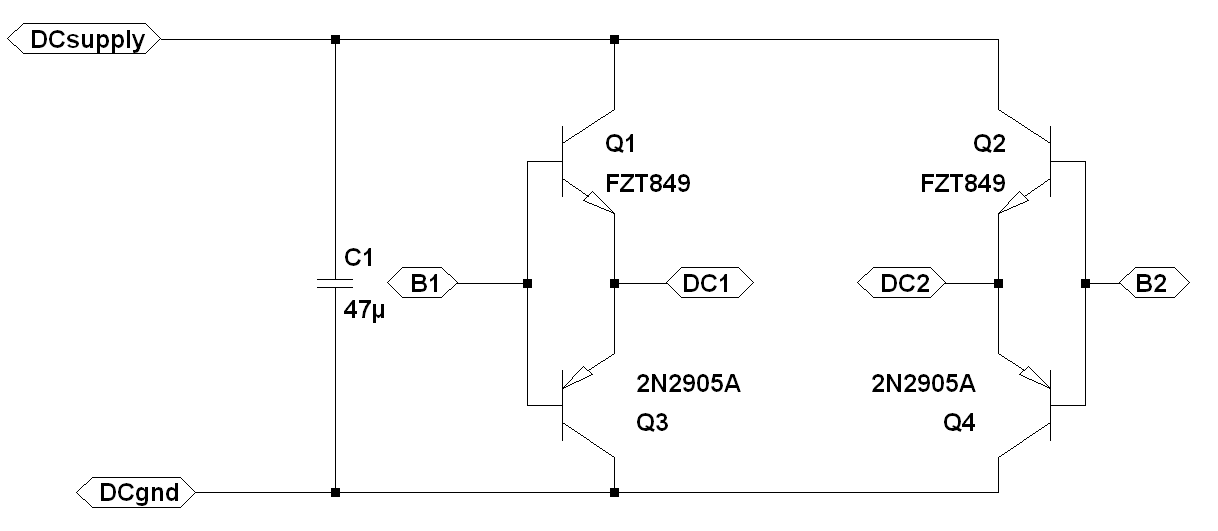
\includegraphics[width=0.8\textwidth]{./img/motor_driver}
  \caption{Complete Motor Driver Circuit}
  \label{fig:motor_driver}
\end{figure}
From Figure~\ref{fig:motor_driver}, it can be observed that only half of the
BJT transistors are in action for a given direction (the other two BJTs are in
cutoff mode). Therefore, a
simplification can be made, which is shown in Figure~\ref{fig:half_mot}. Since
the mode of the two transistors is in active mode, yet another simplification
can be made using dependent sources, shown in Figure~\ref{fig:simp_mot}. At this point, solving for
$R_B$ is much more straightforward:
\begin{align}
  V_{DC_1}-V_{DC_2}\leq 2[V]
  \\ i_B=\frac{1[A]}{(\beta +1)}\approx 4.98[mA]
  \\ \beta i_B +
  \frac{V_{CC}-V_{BE}-V_{DC_1}}{R_B}=\frac{V_{DC_1}-V_{DC_2}}{R_M}
  \\ \frac{V_{DC_1}-V_{DC_2}}{R_M}\leq 1[A]
  \\  \text{Assuming } V_{DC_1}=6[V], V_{DC_2}=4[V]
  \\ R_B =
  \frac{V_{CC}-V_{BE}-V_{DC_1}}{i_B}=\frac{(10-0.8-6)[V]}{4.98[mA]}=642[\Omega]
\end{align}
%image of half of circuit
\begin{figure}[ht!]
  \centering
\begin{circuitikz}\draw
  (0,4) node[anchor=east]{$V_{CC}$}
  to[short,o-*](1,4)
  to [R, l=$R_B$,*-](1,2)
  (3,2)node[npn](npn1){}
  (6,0.5)node[pnp,xscale=-1](pnp1){}
  (npn1)node{$Q_1$}
  (npn1.base)--(1,2)
  (npn1.collector)--(3,4)
  to[short](1,4)
  (npn1.emitter)to[R, l=$R_M$,i=$I_{DC}$](pnp1.emitter)
  (pnp1)node{$Q_2$}
  (pnp1.collector)node[ground]{}
  (pnp1.base)--(8,0.5)
  to [R, l=$R_B$](8,-1)node[ground]{}
;\end{circuitikz}
\caption{Simplified Model of Circuit}
\label{fig:half_mot}
\end{figure}
%image of model
\begin{figure}[ht!]
  \centering
  \begin{circuitikz}\draw
  (0,4) node[anchor=east]{$V_{CC}$}
  to[short,o-*](1,4)
  to [R, l=$R_B$,*-,i=$i_{B}$](1,2)
  to [Do, l=$V_{BE}$,-*](4,2)
  (4,1.6)node[]{$V_{DC_1}$}
  (8.2,2.4)node[]{$V_{DC_2}$}
  (4,4)--(1,4)
  (4,4)to[american controlled current source,l=$\beta i_{B}$](4,2)
  (4,2)to[R, l=$R_M$,i=$I_{DC}$](8,2)
  (8,2)to[Do, l=$V_{BE}$,*-](11,2)
  (11,2)to[R,l=$R_B$,i=$I_{B}$](11,0)node[ground]{}
  (8,2)to[american controlled current source,l=$\beta
  i_{B}$](8,0)node[ground]{}
;\end{circuitikz}
\caption{Further Simplified Model of Circuit}
\label{fig:simp_mot}
\end{figure}
\newpage 
\subsection{$R_B$ by simulations}
Using LTSpice, the circuit found in Figure~\ref{fig:motor_driver} was built and
then tested to see if it in fact would provide the required 1 Amp across the
loading terminals. The test circuit is shown below in
Figure~\ref{fig:motor_driver_t}. Note that $X_1$ is the circuit in
Figure~\ref{fig:motor_driver}. Using the calculated $R_B$, the current through
$R_M$ was found to be $853[mA]$. The voltage $V_{DC_1}$ was found to be
$6.7[V]$ and $V_{DC_2}$ was found to be $5V$. Their difference was
$1.7[V]$. While not ideal, this setup fulfills the required functionality. From
this model, the power dissipated by the transistors can be calculated using
Equation~\eqref{transpower}.

\begin{equation}
  P[W]=(V_C-V_E)I_{DC}\approx2.81[W]
  \label{transpower}
\end{equation}

From this expression, up to about 3 Watts of power will course through the BJTs,
which is why heat sinks are used to prevent the transistors from breaking down
after extensive operation.

\begin{figure}[ht!]
  \centering
  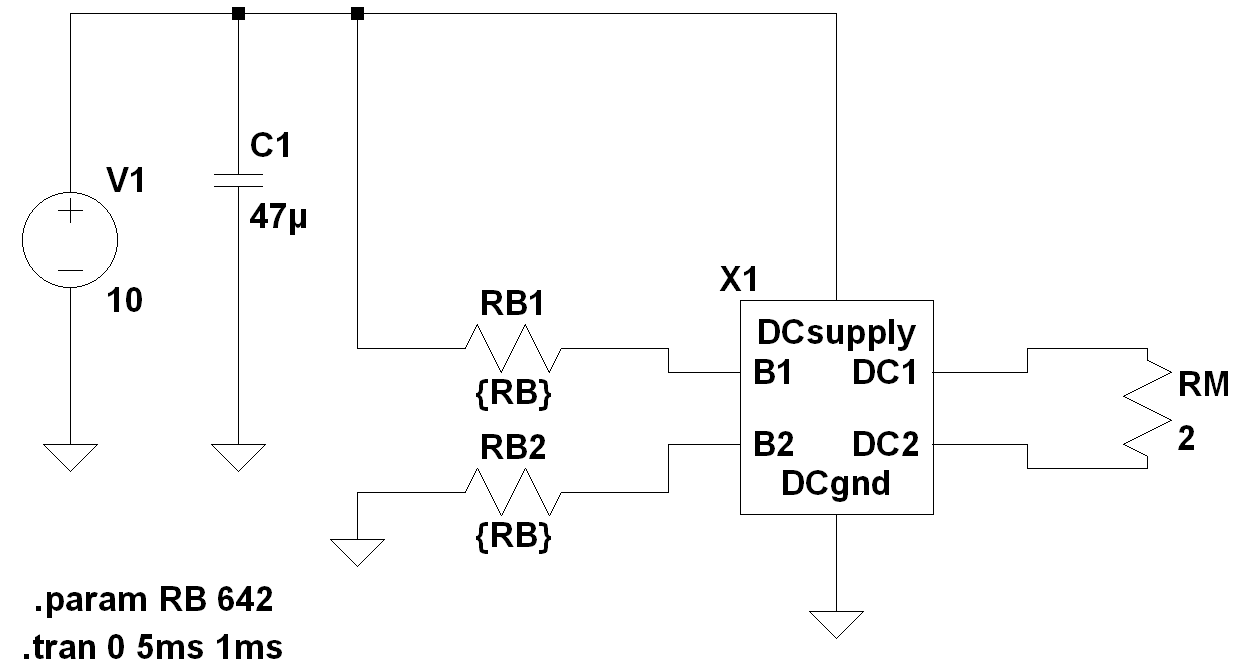
\includegraphics[width=0.8\textwidth]{./img/motor_driver_t.png}
  \caption{Motor Driver Circuit Test}
  \label{fig:motor_driver_t}
\end{figure}
\subsection{$R_B$ by experiment}
Using the actual board, the same values were measured by holding the wheel in
place and taking measurements. The resistor used was a pair of $642[\Omega]$
resistors.
\begin{itemize}
  \item Locked; Clockwise configuration: $I_{DC}=880[mA]$
  \item Locked; Counter-Clockwise configuration: $I_{DC}=870[mA]$
  \item Either Direction Free-Rolling; $I_{DC}=150[mA]$; Speed is $962[Hz]$ = $7.87[rot/s]$ 
\end{itemize}
    Some adjustments to $R_B$ were made throughout the expirement,
    but the most accurate and reliable found was the original 
    $642[\Omega]$ resistors
    calculated in previous sections.
\part{Closed-Loop Motor Driver Circit}
  In this part of the lab, we constructed and tested the complete 
  speed control circuit for a single wheel. The overall schematic 
  for the speed control unit is shown below as
  Figure~\ref{fig:overall}. This circuit is a feedback circuit,
  and can be diagramed as such in Figure~\ref{fig:overall2}.

  \begin{figure}[ht!]
    \centering
    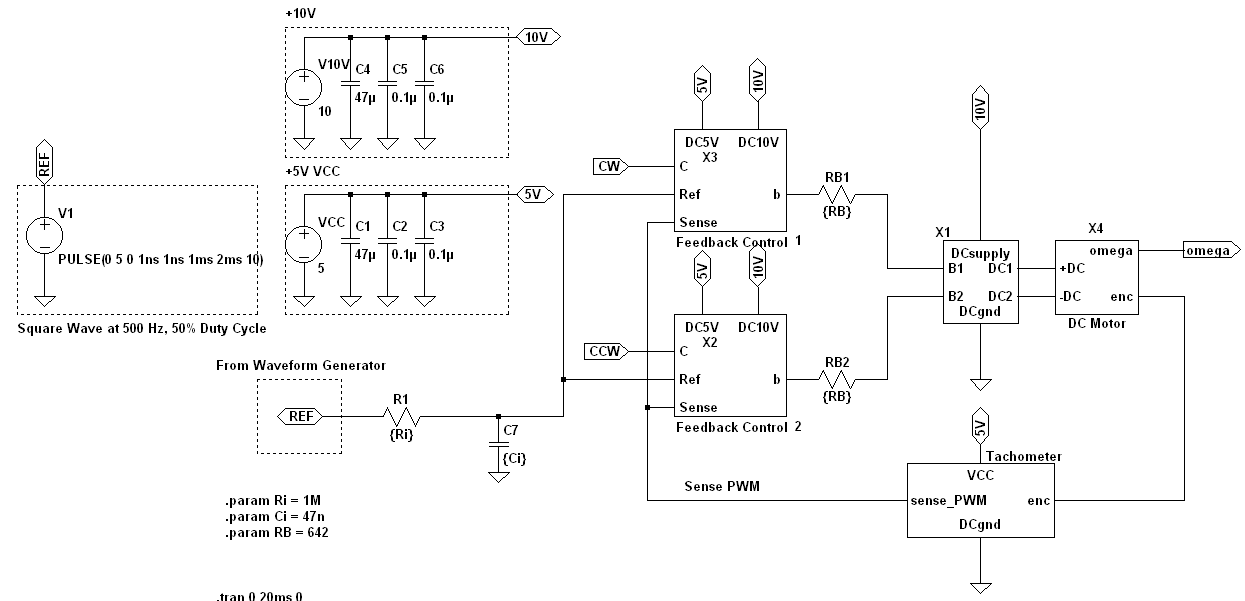
\includegraphics[width=\textwidth]{./img/overall.png}
    \caption{The Total Speed Control Schematic}
    \label{fig:overall}
  \end{figure}
  \begin{figure}[ht!]
    \centering
    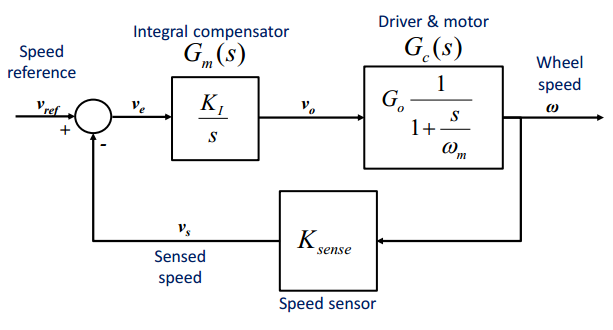
\includegraphics[width=0.6\textwidth]{./img/overall2.png}
    \caption{System Schematic of Circuit}
    \label{fig:overall2}
  \end{figure}
  Of the parts in Figure~\ref{fig:overall2}, we have already built
  the Speed Sensor and the Driver/Motor units. The remaining part
  is the integral compensator, which serves the important role of
  improving steady-state error characteristics. This is done by
  adding a pole at the origin of the complex plane.
  \newpage
\section{Integral Compensator}
% What we did 9/30 and 10/3
We built the Integral compensator, shown below in
Figure~\ref{fig:integralcomp}.

We used the original low-pass filter components $R_3$ and $C_3$ as 
an initial set of starting values. However, the integral 
compensator is not an isolated part of the circuit; its output in 
turn will affect its own input. Using a function generator for 
$V_{ref}$ with a square wave amplitude $0-5[V]$, with a frequency 
of $1[kHz]$, we varied the duty cycle and found that the
wheel's speed was proportional to the percent time on for
$V_{ref}$. Ideally, the wheel speed would reach the highest speed
possible. However, because $t_{on}=\frac{3}{4 f_{enc}}$, the
highest PWM duty cycle is limited, meaning the final speed is some
fraction of the maximum encoder frequency $f_{enc}$, which was
measured previously as approximately $1.2$[kHz].

The transfer function for the integral compensator $G_m(s)$ is derived
below:

\begin{align*}
  v_n = v_p
  \\ i_n = i_p \approx 0
  \\ \frac{v_s-v_n}{R_I} - \frac{v_n-v_o}{\frac{1}{s C_I}} &= 0
  \\ \frac{v_{ref}-v_p}{R_I}-\frac{v_p}{\frac{1}{s C_I}}&=0
  \\ v_o(s) &= \frac{v_{ref}-v_s}{s R_I C_I}
  \\ K_I &= \frac{1}{R_I C_I}
  \\ G_m(s) &=\frac{K_I(v_{ref}-v_s)}{s}
\end{align*}

\begin{figure}[ht!]
  \centering
  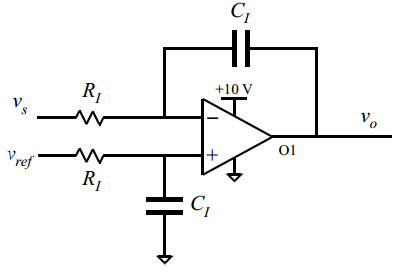
\includegraphics[width=0.4\textwidth]{./img/integralcomp.png}
  \caption{Integral Compensator}
  \label{fig:integralcomp}
\end{figure}

\section{Transient Response}
The integral compensator, however, would not necessarily work with
the values used for $R_3$ and $C_3$ used in the Low-Pass Filter of 
Lab 2. This is because the feedback system gives rise to a Second-
Order system. Our next task was to find a better value for $R_I$
and $C_I$. 
As seen in Figure~\ref{fig:transient}, we had to first
seek out values for $C_I$ and $R_I$ that would not violate
parameters from previous labs, but also be critically damped, that
is, have a $\zeta=1$. In order to calculate this, we have to find
$G(s)$ and then set up the expression to solve for $\zeta$ seen in
Equation~\eqref{eq:transferfunc}.

\begin{equation}
  \frac{v_o(s)}{v_{ref}(s)}=G(s)=\frac{H_0}{1+2\zeta\frac{s}{\omega_0}+(\frac{s}{\omega_0)^2}}
  \label{eq:transferfunc}
\end{equation}

Also, given in the lectures, we have important values $K_{sense}$
and $\omega_0$.

\begin{align*}
  K_{sense} &= \frac{V_{s_{max}}*12*64}{2 \pi f_{enc_{max}}}
  \\ \omega_0 &= \sqrt{\frac{k K_I K_{sense}}{J R_I}}
\end{align*}



\begin{align*}
  \zeta = \frac{1}{2} k \sqrt{\frac{k}{K_I K_{sense} J R_I}}
\end{align*}

\begin{figure}[ht]
  \centering
  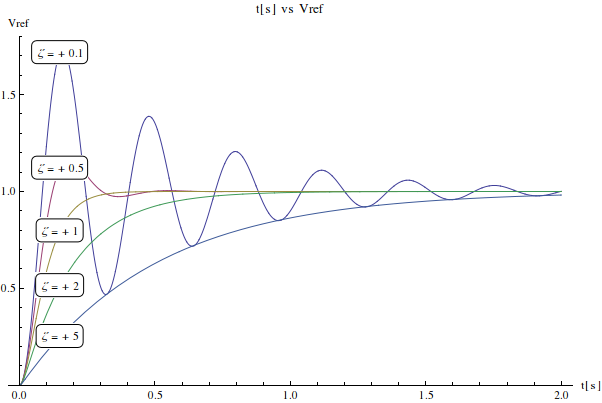
\includegraphics[width=0.9\textwidth]{./img/damping.png}
  \caption{Transients and $\zeta$}
  \label{fig:transient}
\end{figure}

% Solving for a good zeta and why its important
\subsection{$w$ vs $V_{ref}$ for CW and CCW Operation}
% Two-pane table of each plot

\subsection{$K_{sense}$}
\subsection{Derivation of Closed-Loop Transfer Function $G(s)$}
\subsection{Poles of $G(s)$}
\subsection{Step Response Evaluation}
\subsection{Response time of the Speed Controller}
% Plot
\section{Stop and Go Control}
Using a PMOS transistor, with the Source tied to $5[V]$, the Drain to the point
after the $R_I$ on the negative terminal on the op amp
% Prepare demo setup, get a cleaner circuit that looks
% like the circuit in Lecture06.pdf

\end{document}
